\documentclass[10 pt,usenames,dvipsnames, oneside]{article}
\usepackage{../../../modelo-ensino-medio}



\begin{document}

\begin{center}
  \begin{minipage}[l]{3cm}

\includegraphics[width=2cm]{logo}    
\end{minipage}\hfill
\begin{minipage}[r]{.8\textwidth}
 {\Large \scshape Atividade: Leis de De Morgan}  
\end{minipage}
\end{center}
\vspace{.2cm}

\ifdefined\prof
%Habilidades da BNCC
\begin{objetivos}
\item a
\end{objetivos}

%Caixa do Para o Professor
\begin{goals}
%Objetivos específicos
\begin{enumerate}
\item Reconhecer propriedades importantes de operações com conjuntos, envolvendo união, interseção e complementação.
\end{enumerate}
\end{goals}

\bigskip
\begin{center}
{\large \scshape Atividade}
\end{center}
\fi

Verifique, usando diagrama de Venn, as seguintes igualdades, conhecidas como as Leis de De Morgan. Sejam \(A\) e \(B\) dois conjuntos, então
\begin{enumerate}
\item {} 
\(\displaystyle{\overline{A\cap B}}=\overline{A}\cup \overline{B}\)

\item {} 
\(\overline{A\cup B}=\overline{A}\cap \overline{B}\)

\end{enumerate}

\ifdefined\prof
\begin{solucao}

Veja a figura a seguir. No primeiro diagrama foi pintada a região correspondente ao complementar da interseção de $A$ e $B$. No segundo diagrama foi realçada em listras vermelhas a região que corresponde ao evento $\overline{A}$ e em listras azuis a região que corresponde ao evento $\overline{B}$. Depois, em cinza foi destacada a região correspondendo à união dos dois. Verifique que correspondem à mesma região.
\begin{figure}[H]
\centering

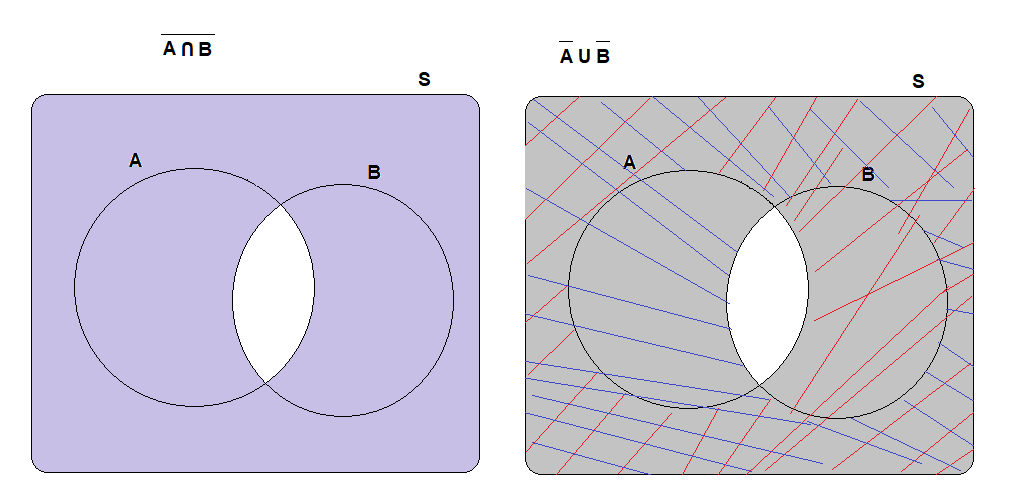
\includegraphics[width=.7\linewidth]{demorgan1.png}

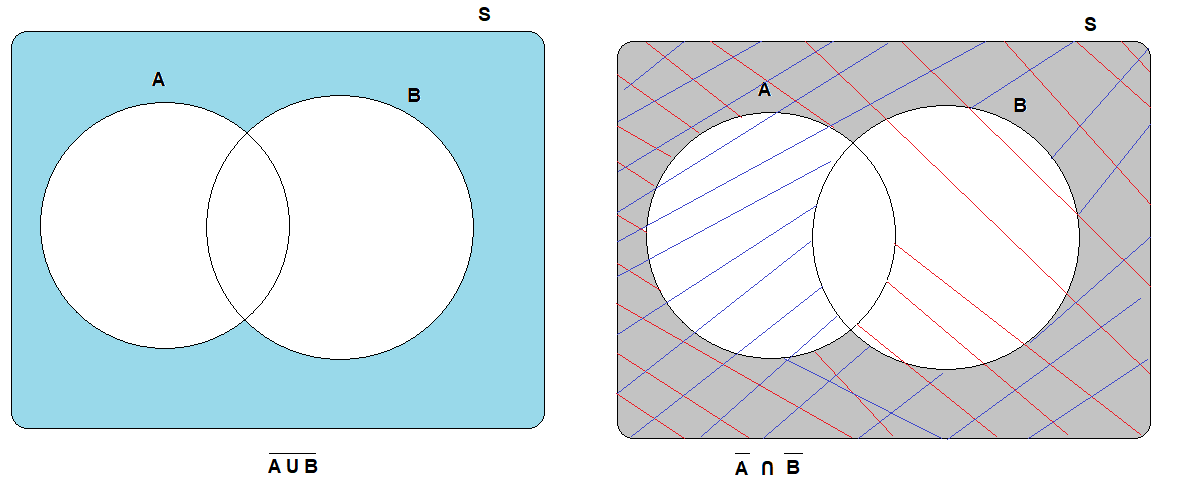
\includegraphics[width=.7\linewidth]{demorgan2.png}
\caption{As leis de De Morgan podem ser enunciadas da seguinte forma:}
\label{}
\end{figure}

\begin{enumerate}
\item O complementar da interseção de dois eventos é igual a união dos complementares desses dois eventos.
\item O complementar da união de dois eventos é igual a interseção dos complementares desses dois eventos.
\end{enumerate}
\end{solucao}
\fi

\end{document}